\onecolumn
\begin{table}[]
    \centering
        \begin{tabular}{lll}
        & Potassium & Calcium\\
        RTC & 
        \includegraphics[width=.45\linewidth,valign=m]{1/K_RTC_.png} & 
        \includegraphics[width=.45\linewidth,valign=m]{1/Ca_RTC_.png} \\ 
        Gillespie & 
        \includegraphics[width=.45\linewidth,valign=m]{1/K_GILLESPIE_.png} & 
        \includegraphics[width=.45\linewidth,valign=m]{1/Ca_GILLESPIE_.png} \\ 
        \end{tabular}
    \caption{Heatmap of the RTC and Gillespie representations using one channel for each type}
    \label{tab:my_label}
\end{table}

\begin{table}[]
    \centering
    \begin{tabular}{lll}
        & Potassium & Calcium\\
        RTC & 
        \includegraphics[width=.45\linewidth,valign=m]{10/K_RTC_.png} & 
        \includegraphics[width=.45\linewidth,valign=m]{10/Ca_RTC_.png} \\ 
        Gillespie & 
        \includegraphics[width=.45\linewidth,valign=m]{10/K_GILLESPIE_.png} & 
        \includegraphics[width=.45\linewidth,valign=m]{10/Ca_GILLESPIE_.png} \\ 
    \end{tabular}
    \caption{Heatmap of the RTC and Gillespie representations using ten channels for each type}
    \label{tab:my_label}
\end{table}


\begin{table}[]
    \centering
    \begin{tabular}{lll}
    & Potassium & Calcium\\
    RTC & 
    \includegraphics[width=.45\linewidth,valign=m]{50/K_RTC_.png} & 
    \includegraphics[width=.45\linewidth,valign=m]{50/Ca_RTC_.png} \\ 
    Gillespie & 
    \includegraphics[width=.45\linewidth,valign=m]{50/K_GILLESPIE_.png} & 
    \includegraphics[width=.45\linewidth,valign=m]{50/Ca_GILLESPIE_.png} \\ 
    \end{tabular}
    \caption{Heatmap of the RTC and Gillespie representations using fifty channels for each type}
    \label{tab:my_label}
\end{table}

\begin{table}[]
    \centering
    \begin{tabular}{lll}
    & Potassium & Calcium\\
    RTC & 
    \includegraphics[width=.45\linewidth,valign=m]{100/K_RTC_.png} & 
    \includegraphics[width=.45\linewidth,valign=m]{100/Ca_RTC_.png} \\ 
    Gillespie & 
    \includegraphics[width=.45\linewidth,valign=m]{100/K_GILLESPIE_.png} & 
        \includegraphics[width=.45\linewidth,valign=m]{100/Ca_GILLESPIE_.png} \\ 
    \end{tabular}
    \caption{Heatmap of the RTC and Gillespie representations using one hundred channels for each type}
    \label{tab:my_label}
\end{table}

